In this section we will review the way the pronunciation scoring system works
and explain the concepts and techniques on which it is based. The diagram below
shows the overall architecture of the system:

~

\begin{figure}[H]
	\centering
	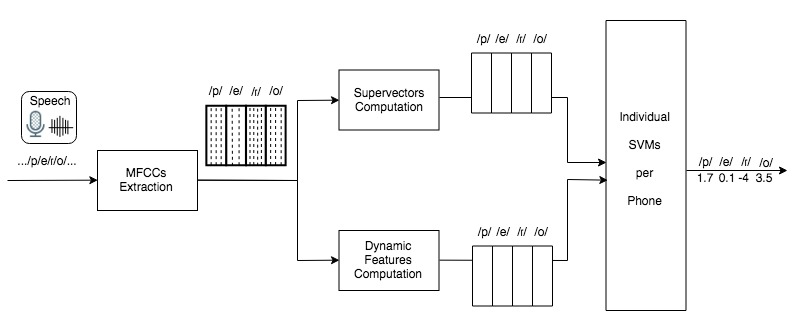
\includegraphics[width=0.9\textwidth]{files/figures/method/general-structure-v2.jpg}
	\caption{General System Architecture}
	\label{fig:methodGeneralArchitecture}
\end{figure}

Given a test instance, the objective is to compute a score for each phone that
is uttered in that instance. In order to do so, the flow goes as follows:

\begin{enumerate}

 \item The first step is to calculate the audio features from the recordings.
 This is done in order to summarize the signal information
 in a measurable way through numeric values. The chosen features
 are the \textit{Mel Frecuency Cepstral Coefficients} (MFCCs) because they are one of the
 most standard and widely-spread features in the speech processing field.

 \item The MFCCs are then split in segments according to the phones to which they
 belong. Each segment is at the same time divided in frames, that represent short
 intervals where the audio signal is not supposed to be changing so much.

 \item MFCCs of each phone instance present in the utterance
 are then used to compute the more complex phone-level features
 on which the SVMs operates. Supervectors are the base and proven to work features,
 while the Dynamic Features are the experimental features to be studied.

 \item {
  SVM classifiers are trained individually for each phone. Two alternative ways of combining the
  features are studied:
    \begin{itemize}
      \item Training a single SVM from a combination of both Supervectors and Dynamic Features.
      \item Training two separate SVMs: one using the Supervector features while the other using the
      Dynamic Features, and then combining the results.
    \end{itemize}
 }

 \item Finally an individual score is obtained for each of the instances
 of the different phones present in the
 utterance. Phone instances with positive score are labelled as
 correct while phone instances with negative score are labelled as incorrect.
 The bigger the magnitude of the score, the more sure the system is about the
 decision.

\end{enumerate}

